\documentclass[a4paper]{article}

\usepackage[ngerman]{babel}
\usepackage[utf8]{inputenc}
\usepackage{enumitem}
\usepackage{amsmath}
\usepackage{array}
\usepackage{graphicx}
\usepackage{xcolor}


\title{Grundlagen der Rechnerarchitektur\\ Übungsblatt 8\\Gruppe 121\\}
\author{Jonas Otto\and Dominik Authaler}

\date{\today}

\begin{document}

\maketitle

\section*{Aufgabe 1}
\section*{Aufgabe 2}
\begin{enumerate}[label=\alph*)]
	\item Wahrheitstabelle: \\
	\begin{tabular}{cccc|c}
		$x_3$ & $x_2$ & $x_1$ & $x_0$ & $f(x)$ \\
		\hline
		0 & 0 & 0 & 0 & 1 \\
		0 & 0 & 0 & 1 & 0 \\
		0 & 0 & 1 & 0 & 0 \\
		0 & 0 & 1 & 1 & 1 \\
		0 & 1 & 0 & 0 & 1 \\
		0 & 1 & 0 & 1 & 0 \\
		0 & 1 & 1 & 0 & 1 \\
		0 & 1 & 1 & 1 & 0 \\
		1 & 0 & 0 & 0 & 1 \\
		1 & 0 & 0 & 1 & 1 \\
		1 & 0 & 1 & 0 & 0 \\
		1 & 0 & 1 & 1 & 0 \\
		1 & 1 & 0 & 0 & 1 \\
		1 & 1 & 0 & 1 & 0 \\
		1 & 1 & 1 & 0 & 0 \\
		1 & 1 & 1 & 1 & 0 \\
	\end{tabular}
	\item
	\begin{equation*}
		f_{DKNF} = \bar{x}_3\bar{x}_2\bar{x}_1\bar{x}_0 + \bar{x}_3\bar{x}_2x_1x_0 + \bar{x}_3 x_2 \bar{x}_2\bar{x}_1 + \bar{x}_3x_2x_1\bar{x}_0 + x_3\bar{x}_2\bar{x}_1\bar{x}_0 + x_3\bar{x}_2\bar{x}_1x_0 + x_3x_2\bar{x}_1\bar{x}_0 
	\end{equation*} 
	
	\item 
	\begin{align*}
	f_{KKNF} =  &(x_3 + x_2 + x_1 + \bar{x}_0) \cdot (x_3 + x_2 + \bar{x}_1 + x_0) \cdot (x_3 + \bar{x}_2 + x_1 + \bar{x}_0) \cdot (x_3 + \bar{x}_2 + \bar{x}_1 + \bar{x}_0) \\ &\cdot (\bar{x}_3 + x_2 + \bar{x}_1 + x_0) \cdot (\bar{x}_3 + x_2 \bar{x}_1 + \bar{x}_0) \cdot (\bar{x}_3 + \bar{x}_2 + x_1 +\bar{x}_0) \\ &\cdot (\bar{x}_3 + \bar{x}_2 + \bar{x}_1 + x_0) \cdot (\bar{x}_3 + \bar{x}_2 + \bar{x}_1 + \bar{x}_0)
	\end{align*}
	
	\item 
	
	\item Minimierung mittels KV-Diagramm und Überdeckung der Nullen:
%	\begin{align*}
%	\begin{array}{c|c|c|c|c|c}
%	&\bar{x}_0&x_0&x_0&\bar{x}_0&\\
%	\hline
%	\bar{x}_1&1&0&0&1&\bar{x}_3\\
%	\hline
%	x_1&0&1&0&1&\bar{x}_3\\
%	\hline
%	x_1&0&0&0&0&x_3\\
%	\hline
%	\bar{x}_1&1&1&0&1&x_3\\
%	\hline
%	&\bar{x}_2&\bar{x}_2&x_2&x_2&\\
%	\end{array}
%	\end{align*}

	\begin{figure}[h!]
		\begin{center}
			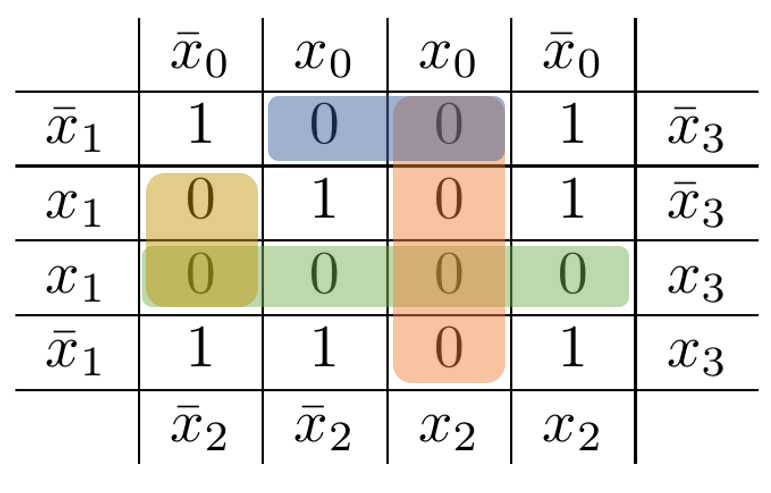
\includegraphics[scale=0.25]{KV_Diagramm_inv.png}
		\end{center}
		\caption{KV-Diagramm zur Minimierung}
	\end{figure}

	\begin{equation*}
	f_{min} = \neg(x_3x_1 + x_2x_0 + \bar{x}_3x_1x_0 + \bar{x}_2x_1\bar{x}_0)
	\end{equation*} 

\end{enumerate}
\section*{Aufgabe 3}
\begin{enumerate}[label=\alph*)]
	\item 
	\item 
	\item Bei CMOS Schaltungen (C für complementary) werden NMOS und PMOS Transistoren gezielt kombiniert, um die Verlustleistung der Schaltung zu verringern und damit ihre Energieeffizienz zu steigern. Dabei wird ausgenutzt, dass die beiden Transistortypen ein komplementäres Schaltungsverhalten aufweisen. Wird der Signalausgang einer Schaltung mit einer der beiden Versorgungsschienen (VCC bzw. GND) verbunden, so wird in der CMOS Schaltungstechnik dafür gesorgt, dass mittels des komplementären Schaltungsverhaltens die Verbindung zur anderen Versorgungsschiene getrennt wird. 
\end{enumerate}



\end{document}
	
